\begin{abstract}
A model can become more likely to answer correctly while producing fewer
kinds of correct answers. This distinction matters for reasoning systems that
sample candidates for verification, search, or revision: a verifier can select
only from the alternatives the model still proposes. We introduce \mb{},
five executable domains whose validators return both correctness and a
canonical solution identity. Its metrics separate finding a correct answer
from finding distinct verified solutions. We then introduce ReplayMaxRL,
which combines MaxRL on fresh samples with replay balanced over previously
discovered solution identities. Across three model scales, verified replay
improves held-out success and sampled support relative to Dr.GRPO. It also
adds to MaxRL at both fully evaluated scales; the partial 3B comparison
remains descriptive. A harder matched benchmark tests the same intervention
beyond the initial task level. Together, the results show that learning to
succeed and maintaining verified alternatives are distinct training goals,
and that explicit memory can help with both.
\end{abstract}

\begin{figure}[H]
  \centering
  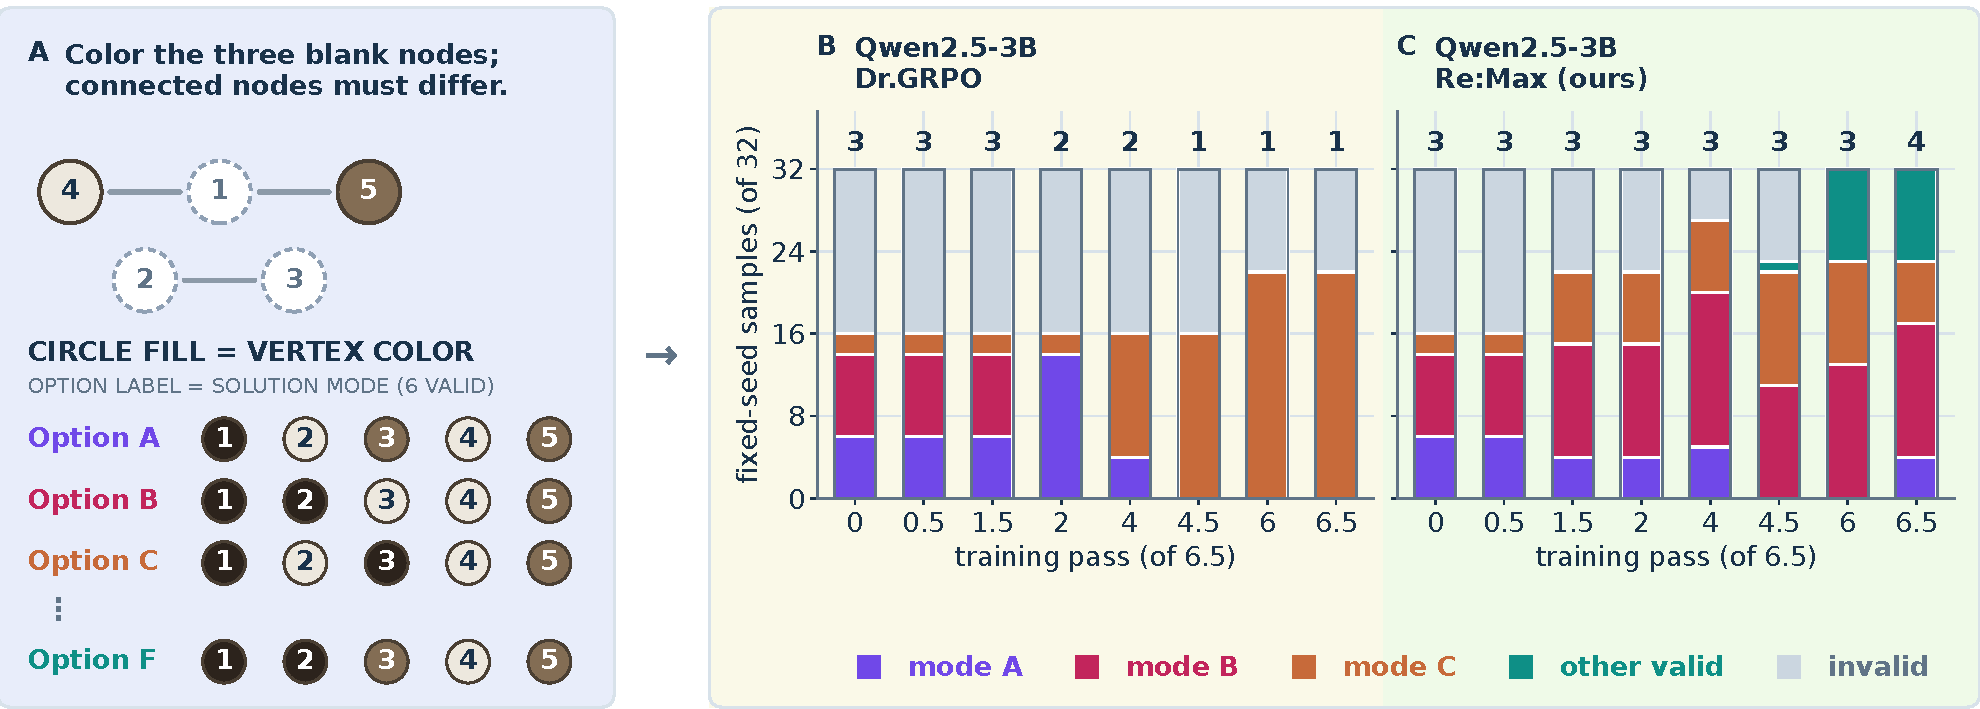
\includegraphics[width=\linewidth]{figures/modecollapse_story.pdf}
  \caption{\textbf{More correct samples can contain fewer distinct solutions.}
  (A) One Graph prompt admits multiple valid colorings. Vertex fill denotes
  color; dashed rings mark the missing vertices; labels identify solution modes.
  (B--C) Matched Qwen2.5-3B runs begin with the same sampled support. Dr.GRPO
  concentrates on one coloring as correctness improves, while ReplayMaxRL
  samples several. Each bar pools four fixed $K=8$ draws; numbers above bars
  count unique verified keys. This is one illustrative prompt, with the
  full collapse precheck in Appendix~\ref{app:pre-rl-regression}.}
  \label{fig:story}
\end{figure}

\section{Introduction}
\label{sec:introduction}

Reinforcement learning with verifiable rewards (RLVR) teaches a model to
produce outputs that pass an executable check \citep{guo2025deepseekr1}.
But the reward need not distinguish two different solutions from two copies
of the same solution. A policy can therefore improve its chance of success
while concentrating its correct outputs on fewer behaviors. Figure~\ref{fig:story}
shows the distinction directly: more successful samples need not mean more
ways of succeeding.

This matters for reasoning systems that generate candidates, verify them,
and revise after feedback \citep{brown2024monkeys,snell2024testtime}.
Search depends on the proposals it receives. Distinct verified routes could
provide alternatives when an approach fails or constraints change, although
that downstream benefit is not established by counting modes alone. Our
question concerns the proposal distribution itself: which verified
alternatives remain available after training?

Answering it requires a definition of solution identity. Different strings
can implement the same computation, while different computations can reach
the same answer. Entropy and string diversity do not resolve this distinction.
\mb{} uses execution to return a canonical key for each accepted output.
Aliases share a key; task-defined behavioral differences receive different
keys. This lets us measure whether training finds a correct output and
whether it finds multiple distinct correct outputs, on the same prompts.

The same identity can guide a memory. Fresh on-policy learning updates from
what the model currently samples; a rare mode may contribute little or no
signal. ReplayMaxRL stores policy-generated verified exemplars and revisits
their keys with equal weight, alongside MaxRL updates on fresh samples
\citep{tajwar2026maxrl}. Deduplicating by key prevents a frequently rediscovered
solution from occupying the memory repeatedly. The intervention asks whether
continued learning from past verified solutions adds value beyond improving
fresh-rollout success.

We contribute an executable benchmark, a replay method, and a controlled
test of this distinction. The experiments first add replay to Dr.GRPO across
model scales, then test it alongside MaxRL, and finally repeat the factorial
at a harder matched level. The evidence supports broader held-out sampled
support under replay. It does not establish that every stored mode survives,
or that broader support causes the accompanying correctness gains.

\section{Related Work}
\label{sec:related}

\noindent\textbf{Diversity under verifiable learning.}
Prior work reports reduced output diversity under RLHF or reasoning RL,
declining entropy, and reduced high-budget problem coverage
\citep{kirk2024understanding,dang2025diversity,cui2025entropy,yue2025rlvrlimit}.
These measurements differ from the within-prompt verified behaviors studied
here. Semantic clustering infers equivalence \citep{farquhar2024detecting};
\mb{} defines identity through accepting execution.

\noindent\textbf{Exploration and memory.}
Outcome bonuses, set objectives, and uniform-correct objectives encourage
broader fresh-sample support
\citep{song2025outcome,chen2025passktraining,li2026setpo,lochab2026ucpo}.
MaxRL combines success objectives across sampling budgets
\citep{tajwar2026maxrl}. Replay reuses experience and can mitigate forgetting
\citep{lin1992selfimproving,rolnick2019replay}; RLEP replays successful reasoning
trajectories \citep{zhang2025rlep}. Quality-diversity methods retain solutions
by behavioral descriptor \citep{mouret2015illuminating}. ReplayMaxRL brings
these ideas together through execution-key memory inside RLVR, and tests
its contribution with matched fresh objectives and replay controls.

\section{Correctness and Verified Support}
\label{sec:collapse}

For a prompt $x$, let the validator $V_x(y)$ return either a verified solution
key $c\in\mathcal C_x$ or failure $\bot$. The learner observes keys only for
responses it generates; it receives neither the full valid set nor a list
of target solutions. A policy induces a total success probability and a
conditional distribution over correct keys. We call concentration of that
conditional distribution onto fewer keys \emph{mode collapse}. Correctness
alone cannot reveal it.

\subsection{Measuring success and support}
\label{sec:collapse-metrics}

For $K$ independent samples, let $D_K$ count their distinct verified keys.
Our two primary measurements are
\[
  \texttt{pass@}K=\Pr[D_K>0],
  \qquad
  \texttt{distinct@}K=\E[D_K].
\]
The first asks whether sampling finds any correct output. The second asks
how many distinct correct outputs it finds. Their units differ: probability
versus an expected key count. We report them together at a fixed budget
$K=8$, without treating equal numerical changes as equivalent gains.

To interpret a support increase, we also report
$\texttt{distinct@}K-\texttt{pass@}K$: the expected number of verified keys
beyond the first. This decomposition helps distinguish gaining a first
success from sampling additional solutions. It remains affected by the
number of successful draws, so it is not a fully success-matched diversity
measure. Neither metric recovers the full positive-probability support from
finite samples. Appendix~\ref{app:metric-details} gives the sampling identities,
reference policies, and diagnostic per-sample correctness metric.

\subsection{Why fresh rewards can favor common modes}
\label{sec:collapse-mechanism}

GRPO and Dr.GRPO center rewards within a sampled group
\citep{shao2024deepseekmath,liu2025understanding}. Equally correct outputs
receive the same task credit regardless of key, but common modes appear in
more groups. A categorical model makes this feedback explicit. With
independently trained softmax logits, expected binary-reward gradient ascent
satisfies, for two correct modes $c,d$,
\[
  \frac{d}{dt}\log\frac{p_c}{p_d}=(p_c-p_d)(1-P),
\]
where $P$ is total correct probability. While incorrect mass remains, an
existing advantage in frequency grows. The mean group estimators, including
binary MaxRL, share this direction up to a positive speed factor; finite
groups also provide no direct score term for an unsampled mode.
Appendix~\ref{app:theory} states the assumptions and proves the resulting
collapse claim. This idealized calculation motivates a memory that supplies
training signal even when an exemplar is absent from the fresh group.

\section{\mb: Executable Modes Across Levels}
\label{sec:modebench}

\mb{} makes a mode an auditable property of execution. Each validator both
accepts a response and returns its canonical identity. Surface aliases merge;
differences meaningful to the task remain. Figure~\ref{fig:modebench-examples}
shows the five domains and the resulting keys.

\begin{figure}[H]
  \centering
  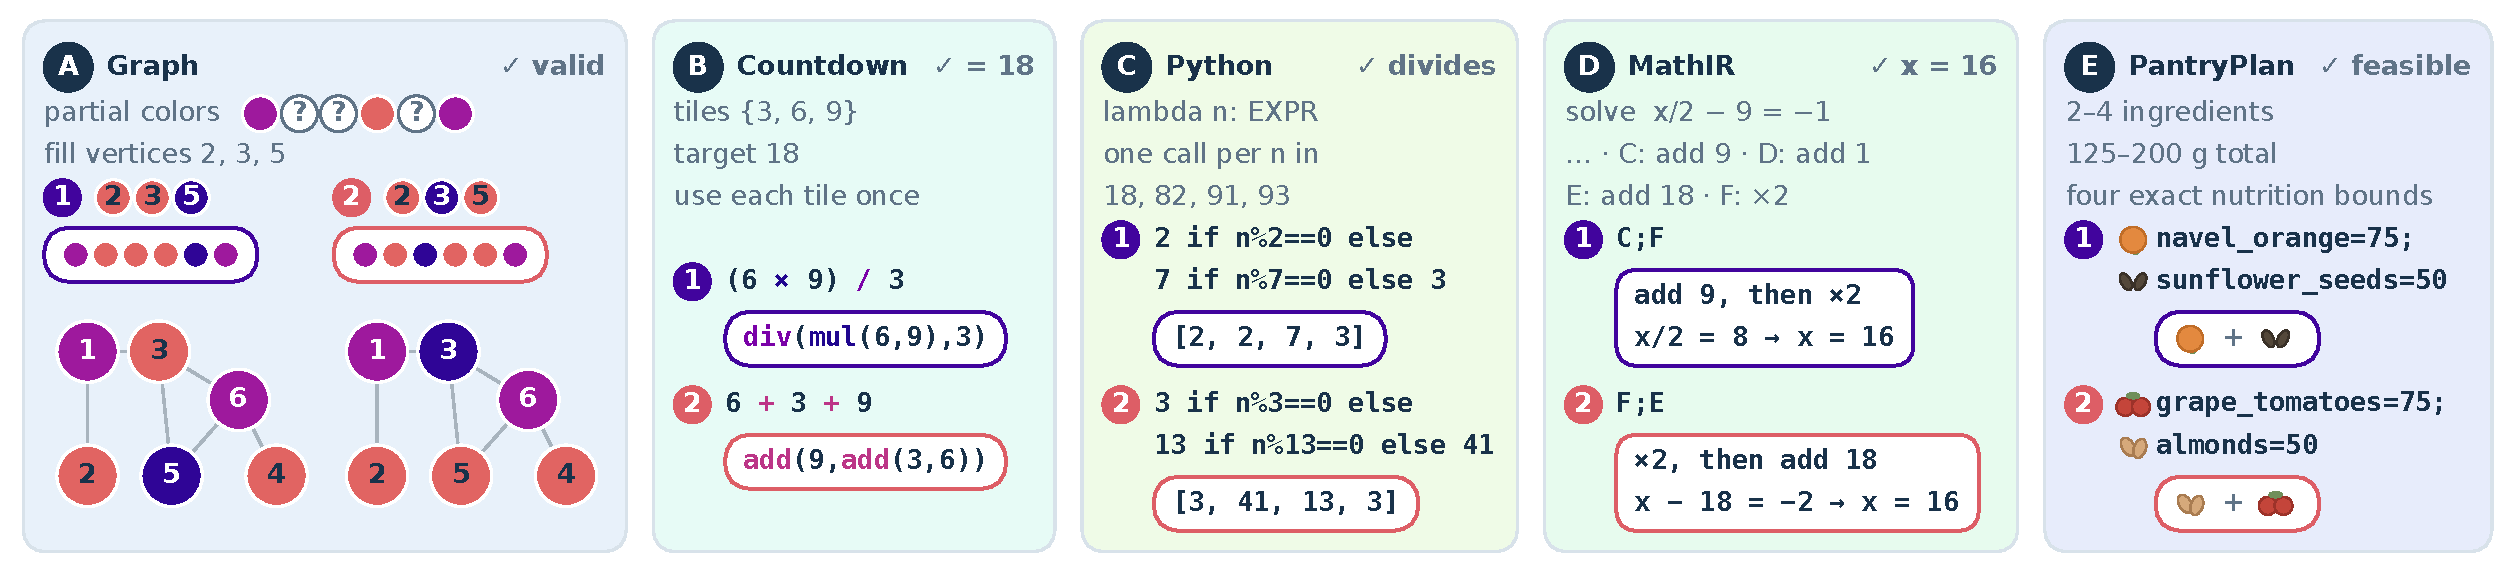
\includegraphics[width=\linewidth]{figures/modebench_examples.pdf}
  \caption{\textbf{Execution distinguishes verified solutions from surface variants.}
  Each panel shows two correct responses and their distinct canonical keys.
  Graph and PantryPlan keys identify valid configurations; Countdown and
  MathIR identify computation or derivation routes; Python identifies behavior
  on frozen inputs. These are task-specific notions of difference, rather
  than a universal measure of reasoning diversity.}
  \label{fig:modebench-examples}
\end{figure}

Graph coloring identifies a complete color assignment. Countdown identifies
a normalized arithmetic computation tree. Python factors identifies the
return vector of an executed program, merging programs with the same observed
behavior. MathIR identifies a normalized trajectory of algebraic states.
PantryPlan identifies a feasible ingredient support, merging quantity and
ordering aliases. Thus a gain in sampled modes has a concrete, domain-specific
meaning; it need not imply more reasoning routes in every domain.

Each domain has two disjoint difficulty levels with the same validator and
key definition. Level 2 changes problem structure while matching the
training/evaluation valid-mode-count histograms, so harder problems do not
simply offer fewer correct modes. This supports a controlled difficulty test
with unchanged measurement. Appendix~\ref{app:data} specifies the constructions,
mode inventories, splits, and exact prompts; it also documents what each key
can and cannot distinguish.

\section{ReplayMaxRL: Explore and Preserve Verified Modes}
\label{sec:method}

ReplayMaxRL separates learning from fresh samples from revisiting verified
exemplars. Both use the policy's own outputs. Fresh learning rewards success;
the memory uses keys to decide which previously successful outputs to revisit.
Figure~\ref{fig:verified-support-story} shows the two paths.

\begin{figure}[H]
  \centering
  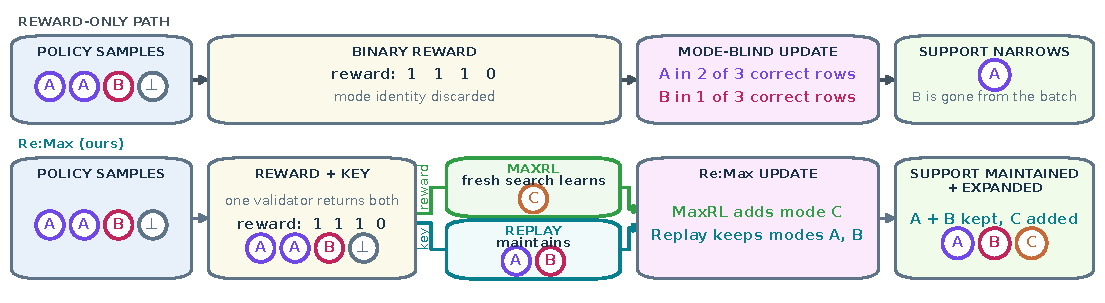
\includegraphics[width=\linewidth]{figures/verified_support_story.pdf}
  \caption{\textbf{Fresh learning and verified memory supply complementary signals.}
  The same rollouts provide binary rewards to MaxRL and canonical keys to the
  replay bank. Fresh learning can discover C while replay revisits stored
  exemplars of A and B. A key receives one bank entry regardless of how often
  it is rediscovered. The schematic describes the update mechanism; actual
  held-out support is measured by the experiments.}
  \label{fig:verified-support-story}
\end{figure}

\subsection{Fresh learning with binary MaxRL}
\label{sec:maxrl-method}

MaxRL weights success across sampling budgets \citep{tajwar2026maxrl}. For
$G$ fresh binary rewards with $m=\sum_i r_i$ successes, we use the advantage
\[
 A_i^{\mathrm{MaxRL}}=
 \begin{cases}Gr_i/m-1,&m>0,\\0,&m=0.\end{cases}
\]
All-failure and all-success groups have zero task advantage. The finite-group
mean objective is derived in Lemma~\ref{lem:maxrl-mean}. These advantages
apply only to fresh on-policy responses; replay rows never enter the group
or its reward statistics.

\subsection{Replay balanced over verified keys}
\label{sec:replay}

Each training prompt owns an initially empty, bounded bank $\mathcal B_x$.
It retains one policy-generated exemplar $e_c$ per admitted verified key,
with no gold solutions or unverified proposals. A round-robin schedule
revisits nonempty prompt banks. Within a bank, the replay loss gives keys
equal weight:
\begin{equation}
 L_\mathrm{replay}(x)=-\frac1{|\mathcal B_x|}
 \sum_{c\in\mathcal B_x}\frac{\log\pi_\theta(e_c\mid x)}{|e_c|}.
 \label{eq:lm-verified-replay}
\end{equation}
This is supervised likelihood learning on verified exemplars, with each
response's log likelihood normalized by its token length. Key balancing
prevents frequently rediscovered solutions from determining the replay
weights. Only training-prompt responses enter the bank.

In an ideal categorical model, uniform-key replay rewards both the total
probability on banked modes and balance within that set
(Appendix~\ref{app:replay-metric-alignment}). At fixed success probability,
balancing mode probabilities increases expected sampled coverage. This
explains the choice of weights without implying that the combined neural
update improves both metrics at every step. A stored response is one
exemplar of a key, not its entire probability mass.

We add this loss to the fresh MaxRL update to obtain ReplayMaxRL; replacing
MaxRL with Dr.GRPO yields ReplayDr.GRPO. Controls execute the same bank and
scoring code with zero replay derivative, while their evolving policies can
build different banks. This makes replay an explicit factor in the experiment.
Appendix~\ref{app:algorithm} gives capacity, coefficient, admission, masking,
and scheduling details. The fixed-bank theory supplies a qualitative
non-extinction result under its stated assumptions, rather than a guarantee
for the implemented neural optimizer or for undiscovered modes.
